\chapter{Protocol}

\section{Experiment navigation}
Once some experiments are in the protocol, by pushing their ``Send to protocol'' button, they can be moved up, moved down, deleted and edited. Figure \ref{fig:protocol} shows the protocol section in the graphical user interface with the containing buttons.

\section{Delete experiment}
To delete an experiment, the experiment has to be selected with a left-mouse click and then it can be deleted by pushing the button ``X'', number 1 in the figure \ref{fig:protocol}.

\section{Move experiment up/down}
To move an experiment up or down, the experiment also has to be selected and than it can be moved by pushing the button ``\(\uparrow\)'', number 2, respective, the button ``\(\downarrow\)'', number 3 in figure \ref{fig:protocol}.

\section{Edit experiment}
To edit an experiment, the experiment has to be selected and then with a right-mouse click a context menu will appear, where the option ``Edit'' has to be selected. To button ``Send to protocol'' now changed its name to ``Save changes'' and the current tab is locked. Now the parameters can be changed and afterwards applied by pushing the button ``Save changes'' or the process can be canceled by pushing the button ``Cancel''.

\section{Repeat protocol}
If it is desired to repeat the whole protocol, the check-box ``Loop'', number 4 in figure \ref{fig:protocol} can be checked.

\section{Preview}
To get a preview of the protocol, the button ``Preview'', number 5 in figure \ref{fig:protocol} can be pushed. The preview will plot the minimal and maximal force/stress and distance limits and a preview of the force/stress and distance values in the graph.

\section{Start and stop}
The protocol can be started by pushing the button ``Run'', number 6, and stopped by pushing the button ``Stop'', number 7 in figure \ref{fig:protocol}. When the protocol stops, either manually or after the last experiment, the experiments in the protocol will be reseted.

\section{Save and load}
It is possible to save a project to a file to load it later. For this, the button ``Save'', number 8 in figure \ref{fig:protocol} can be pushed, to display a file choosing dialog. Loading an experiment works in the same way, except, that a file has to be chosen in the file dialog, which then will be loaded.

\begin{figure}[!ht]
	\centering
		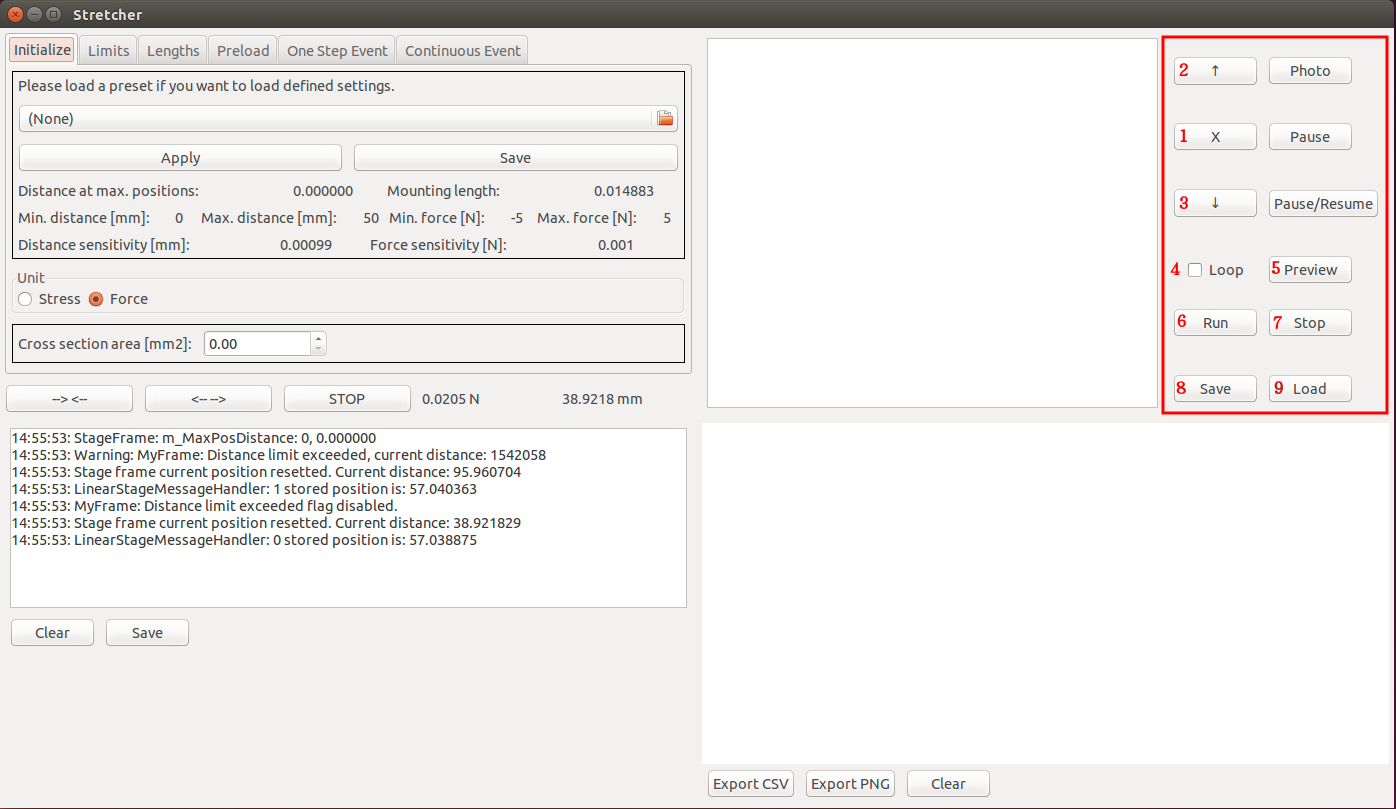
\includegraphics[width=1.0\textwidth]{images/Protocol}
	\caption{Protocol}
	\label{fig:protocol}
\end{figure}
